% =========================================================
% CONFIGURACION DEL DOCUMENTO
% =========================================================
\providecommand{\main}{../..}
\documentclass[\main/main.tex]{subfiles}

% =========================================================
% CONTENIDO
% =========================================================
\begin{document}
\section{Instrumentación y Control}

En el presente capítulo se presentan los procedimientos realizados
para la implementación del control embebido en la planta real. Se
sigue un enfoque modular describiendo por parte cada componente del
sistema, desde la medición de ángulo, la programación de sensores,
la configuración de los controladores electrónicos, los toolkits de
LabVIEW escogidos y las diferentes etapas de experimentación con el
vehículo.

\subsection{Medición de Ángulos}

\subsubsection{Acelerómetro}

Para la medición de los ángulos se utilizan los sensores MEMS descritos
en el capítulo de Componentes del Sistema \ref{Componentes del Sistema}. La mayoría de los acelerómetros
MEMS miden la aceleración por medio de la lectura de capacitancias
variables. Una masa de prueba es puesta entre las placas de los capacitores,
ésta se mueve dependiendo de la aceleración a la que es sometida,
posteriormente se registran las capacitancias, se procesan y entregan
un valor de voltaje proporcional a la aceleración medida. La siguiente
imagen muestra un concepto de lo descrito anteriormente:

\begin{figure}[H]
\noindent \begin{centering}
\includegraphics[scale=0.5]{\string"mems acel\string".jpg}
\par\end{centering}
\caption{Principio físico de funcionamiento de un acelerómetro.}
\end{figure}

Para comprender como estimar los ángulos a partir de las mediciones
de un acelerómetro, es útil imaginar una caja cúbica con una bola
dentro de ella. En primera instancia si la caja estuviera en un lugar
ausente de campos gravitacionales, ninguna fuerza afectaría la posición
de la bola. Por otro lado, si se deja la caja en una superficie plana
sobre la tierra y en reposo, la bola sentiría una aceleración de 1{[}g{]}
hacía la tierra. De lo anterior es claro que de aplicar una fuerza
externa a la caja, la bola se verá afectada por una fuerza ficticia
de igual magnitud y en sentido contrario. Las siguientes imágenes
describen las tres situaciones antes mencionadas.

\begin{figure}[H]
\noindent \begin{centering}
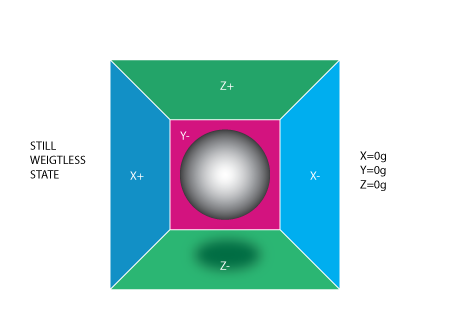
\includegraphics[scale=0.3]{cajabola1}
\par\end{centering}
\noindent \begin{centering}
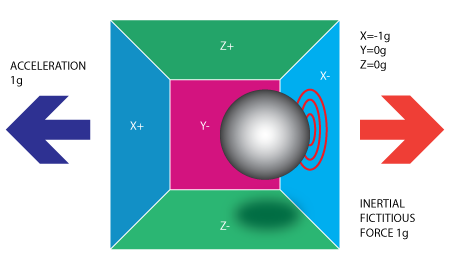
\includegraphics[scale=0.35]{cajabola3}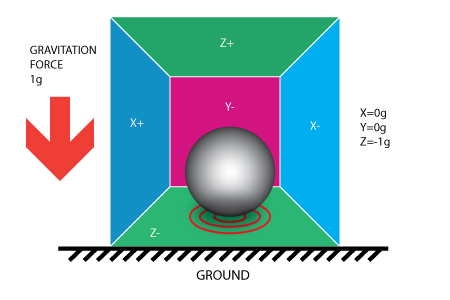
\includegraphics[scale=0.35]{cajabola2}
\par\end{centering}
\caption{Ilustración del funcionamiento de un acelerómetro.}
\end{figure}

Por lo tanto al inducir cualquier rotación sobre la caja e inclinarla,
la bola tendrá asociado un vector de aceleración resultante, que estará
apuntando hacia el centro de la tierra. Dicho vector se puede descomponer
en sus componentes cartesianas $x,\negmedspace y,\negmedspace z$,
con las que es posible calcular el ángulo de inclinación de la caja,
dado que se cuenta con la medición de aceleración en cada componente. 

Antes de estimar los ángulos de inclinación del vehículo, es necesario
mencionar que cualquier acelerómetro es completamente insensible a
rotaciones sobre el vector del campo gravitacional, es decir, si la
caja se encuentra en la superficie terrestre y ésta rota sobre el
eje $z$ de la figura anterior, no es posible utilizar las mediciones
del sensor para estimar dicha rotación (yaw). Por lo tanto con éste sensor sólo
se pueden estiman los ángulos de Pitch y Roll.

Se estudia el efecto de la matriz de rotación al vector del campo
gravitacional de la tierra, inicialmente apuntando en dirección al
eje $z$ con magnitud de 1{[}g{]}. Escribiendo dicho vector en términos
de los ángulos de rotación mediante la matriz descrita en el Capítulo
de Modelado de la Planta \ref{Modelado de la Planta}, se tiene:


\begin{equation}
\left[\begin{array}{c}
x\\
y\\
z
\end{array}\right]=\left[\begin{array}{c}
0\\
0\\
1
\end{array}\right]=[T_{x}][T_{y}][T_{z}]\left[\begin{array}{c}
0\\
0\\
1
\end{array}\right]=\left[\begin{array}{c}
-sin\theta\\
cos\theta sin\phi\\
cos\theta cos\phi
\end{array}\right]\label{eq:rotacion a gravitacional}
\end{equation}

De la representación anterior es claro notar que las componentes $x$
e $y$ del vector aceleración son cero si los anguos de inclinación
son cero y la componente $z$ tiene un valor unitario en el mismo
caso. También es necesario mencionar que la matriz de rotación no
es conmutativa, que el efecto de dicha matriz sobre el campo gravitacional
depende del orden en que rote cada ángulo como se menciona en [17].
Para este trabajo se tomará en cuenta el orden predefinido en el
Capítulo de Modelado de la Planta \ref{Modelado de la Planta} tal como la ecuación (\ref{eq:rotacion a gravitacional})
lo indica, ampliamente utilizada y denominada secuencia de rotación
aeroespacial. Relacionando las componentes normalizadas de la aceleración
medida con los ángulos de elevación pitch y alabeo roll se tiene:

\begin{equation}
\frac{G_{v}}{||G_{v}||}=\left[\begin{array}{c}
-sin\theta\\
cos\theta sin\phi\\
cos\theta cos\phi
\end{array}\right]\implies\frac{1}{\sqrt{G_{x}^{2}+G_{y}^{2}+G_{z}^{2}}}\left[\begin{array}{c}
G_{x}\\
G_{y}\\
G_{z}
\end{array}\right]=\left[\begin{array}{c}
-sin\theta\\
cos\theta sin\phi\\
cos\theta cos\phi
\end{array}\right]
\end{equation}

Resolviendo para pitch $\theta$ y roll $\phi$ se tiene:

\begin{equation}
tan\phi=\frac{G_{y}}{G_{z}}\quad\quad,\quad\quad\hfill tan\theta=\frac{-G_{x}}{\sqrt{G_{y}sin\phi+G_{z}cos\phi}}=\frac{-G_{x}}{\sqrt{G_{y}^{2}+G_{z}^{2}}}
\end{equation}

Por lo tanto los ángulos pitch y roll son:

\begin{equation}
\phi=arctan(\frac{G_{y}}{G_{z}})\quad\quad,\quad\quad\hfill \theta=arctan\left(\frac{-G_{x}}{\sqrt{G_{y}^{2}+G_{z}^{2}}}\right)
\end{equation}

\subsubsection{Gyróscopo}

Para entender como funciona el gyroscopo, es útil imaginar un cuerpo
de masa $m$ moviendose con velocidad $v$. Si se aplica una rotación
angular con velocidad $\Omega$ al cuerpo en movimiento, entonces
éste experimentará una fuerza proporcional al producto cruz de las
velocidades antes mencionadas, como se muestra en la figura \ref{fig:Fuerza-de-coriolis}.
Esta fuerza es conocida como fuerza de Coriolis y su expresión es: 

\begin{equation}
\overrightarrow{F}=2m(\overrightarrow{\Omega}x\overrightarrow{v})
\end{equation}


\begin{figure}[H]
\noindent \begin{centering}
\subfloat[Fuerza de coriolis sobre un cuerpo de masa $m$ a moviendose a velocidad
$v.$\label{fig:Fuerza-de-coriolis}]{\noindent \begin{centering}
\includegraphics[scale=0.5]{\string"coriolis force\string".png}
\par\end{centering}
}\subfloat[Configuración oscilatoria del gyroscopo.\label{fig:Configuracion-oscilatoria-del}]{\noindent \begin{centering}
\includegraphics[scale=0.7]{\string"coriolis force 2\string".png}
\par\end{centering}
}\par\end{centering}
\caption{Principio físico de funcionamiento del gyroscopo.}
\end{figure}

Dado el efecto de la fuerza de Coriolis, el giróscopo mantiene una
masa en constante oscilación como la que se muestra en la figura \ref{fig:Configuracion-oscilatoria-del}.
Luego al aplicar una rotación sobre el sensor, la masa se desplaza
perpendicularmente a la dirección de la velocidad de oscilación, movimiento
que a su vez varia la capacidad de los capacitores internos del sensor
entregando finalmente una medida de voltaje porporcional a la velocidad
de rotación inducida.

Ya que la medición del gyroscopo ITG-3200 utilizado en este proyecto
entrega la velocidad de giro en cada eje en grados por segundo, para
poner medir el ángulo yaw, que el acelerómetro es incapaz de medir, se
integra la medición del gyroscopo con la técnica de integración simple
de Euler hacia atrás. Dado el ruido que introducen los actuadores
sobre la planta, la estimación del ángulo yaw tendrá un error acumulativo
importante, pero no es crítico al momento de sólo estabilizar el sistema,
pues se puede controlar su velocidad directamente. Por lo tanto para
estimar el ángulo yaw del vehículo se hace la siguiente operación:

\begin{equation}
Yz_{k}=Yz_{k-1} + \dot{Yz_{k}}\cdot\Delta t
\end{equation}

Con la medición del gyroscopo $Yz$ en grados
por segundo.

\subsubsection{Consideraciones en Programación}

Para comprobar la estimación de los ángulos obtenida mediante este
proceso, se programa una aplicación en LabVIEW de adquisición de mediciones
del acelerómetro y gyroscopo en el controlador myRIO, junto con una
visualización de un slab en 3D en el computador principal, con el
cual se puede ver directamente el cambio de los ángulos en el tiempo
al inclinar el controlador. En la figura \ref{fig: Slab 3D} se puede apreciar el panel frontal de la aplicación, donde los potenciómetros virtuales son indicadores linkeados a variables de red para comunicar el VI de adquisición que se ejecuta en el dispositivo myRIO, con el VI de visualización que se ejecuta en el PC.
El código de ésta aplicación se incluye
en el apartado de anexos.

\begin{figure}[H]
\noindent \begin{centering}
\includegraphics[scale=0.6]{\string"3D visualzacion slub\string".jpg}
\par\end{centering}
\caption{Aplicación de visualización de ángulos en 3D con LabVIEW.}\label{fig: Slab 3D}\noindent 
\end{figure}

Para el control embebido, tanto el acelerómetro como el gyroscopo
presentan valores de offset distintos de cero. La estrategia adoptada
para eliminar este efecto es que antes de empezar con el loop principal
que ejecuta el algoritmo de control, se programan dos subrutinas que
eliminan ambos offset de los sensores para tener una medición correcta.
Las subrutinas consisten en promediar mil muestras de ambos sensores
con el vehículo en reposo y manteniendolo lo más paralelo al piso
posible, con el fin de restar las componentes de offset del gyróscopo
debido a que está en reposo y repetir el proceso con el acelerómetro
considerando sólo la presencia del campo gravitacional de 1{[}g{]}
en el eje $z$. El código de estas subrutinas se incluye en el Anexo B.


\subsection{Estrategia de Control PID descentralizado}

Para la implementación del control en la planta real se utilizaron
dos estrategias de control lineal, ambas basadas en controladores
PID pero en diferentes configuraciones. 

En primer lugar se programó un control lineal con filtro de ruido
de medición similar al presentado en el capítulo de simulación. La
programación de este controlador se realizó por eje asumiendo el modelo
lineal presentado en el capítulo 3 y se utilizan las constantes
de caracterización de motores para generar la actuación. La variante
que se incluyó para el desarrollo de esta estrategia fue la incorporación
de un filtro pasa bajos determinístico para reducir el ruido de medición,
provocado por los actuadores que inducen vibraciones de alta frecuencia
en la estructura del vehículo. Después de someter a prueba dicha estrategia
de control en cada eje por separado para ambos soportes descritos
en el capítulo de componentes, no se obtuvieron buenos resultados.
La estabilización de la planta no fue posible para ningún eje separadamente,
por lo tanto no se sometió a prueba el sistema completo. El código
de la implementación se adjunta en el Anexo B.

Luego del primer intento con la estrategia de control PID descentralizado,
se decide cambiar la estrategia de control por un control PID en cascada
descentralizado, donde el lazo interior estabiliza la velocidad del
sistema, mientras que el lazo exterior define la posición deseada por
eje. El lazo de control propuesto para la implementación por eje es
la que se propone en [18], tal como se muestra en la figura \ref{pid cascada}.

\begin{figure}[H]
\noindent \begin{centering}
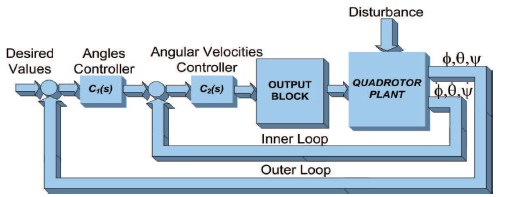
\includegraphics[scale=0.8]{cascada}
\par\end{centering}
\caption{Estrategia de control PID en cascada.}\label{pid cascada}\noindent
\end{figure}

Con esta estrategia de control se logra la estabilización por eje
en ambos soportes, robusto a pequeñas perturbaciones y, en algunos
casos, con un buen seguimiento de referencias constantes.


\subsection{Actuación}


\subsubsection{Configuración del ESC}

En primera instancia se debe aegurar de que los cuatro motores estén
funcionando de la misma forma, vale decir con la misma configuración
del controlador de velocidad ESC. Cabe mencionar que esta parte se
hizo antes de obtener las mediciones de empuje con el banco de pruebas
presentadas en el capítulo de simulación. Dentro de las configuraciónes
más importantes se pueden mencionar la configuración de detención
rápida, aceleración rápida, frecuencia de operación, voltaje de corte
y dirección del giro. Los distintos tipos de configuración del ESC
se adjuntan en el Anexo D junto con el manual. El diagrama
básico de conexión se muestra a continuación:

\begin{figure}[H]
\noindent \begin{centering}
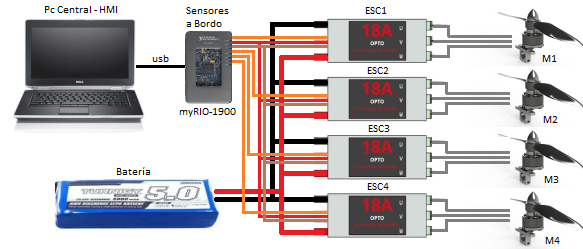
\includegraphics[scale=0.8]{bitmap}
\par\end{centering}
\caption{Diagrama de conexiones del Quadcopter.}
\end{figure}

Por otro lado también es importante mencionar que antes de comenzar
toda prueba, se deben calibrar los motores en el rango de aceleración
que se esté utilizando. Para esto se crean sub VI's que se dedican
a variar uniformemente la señal de control PWM de 50{[}Hz{]} entre
1{[}ms{]} y 2{[}ms{]}, correspondiente a un ciclo de trabajo de un
5\% y un 10\% respectivamente, con la cual el ESC queda configurado
para dar mínima y máxima velocidad de giro a los motores dentro de
ese rango. En el Anexo B se adjunta el código LabVIEW de calibración de motores, mientras que en Anexo D se describe la secuencia de calibración de los cuatro ESC simultáneamente. 

\subsection{Resultados Experimentales}

En esta sección se presentan los resultados experimentales del control
embebido en la planta real. La sección se divide en subsecciones que
describen el funcionamiento por eje en cada soporte, presentando los
resultados de posición angular y actuación en el tiempo. 

A esta estrategia de control se le suma un filtro de ruido de medición
al igual que en la estrategia anterior, puesto que los motores seguirán
generando vibraciones. Las pruebas de estabilización se realizan por
cada eje en los dos soportes adoptando una estrategia de control
diferente a la diseñada en el capítulo 3. La programación
del control embebido con LabVIEW y myRIO se detalla en el Anexo B.

La frecuencia de muestreo escogida para la implementación es de 150[Hz] para todas las pruebas realizadas en ambos soportes.

\subsubsection{Estabilización de Eje Pitch y Roll en Soporte 1}

Para la prueba de estabilización de elevación Pitch se fija el vehículo desde los
dos extremos opuestos del soporte de madera, dejando sólo dos motores
funcionando, aquellos relacionados con el eje en cuestión, tal como se muestra en la figura 5.8.b. Antes de
describir los resultados obtenidos, es necesario comentar que las
pruebas sobre el soporte de madera se hacen con el objetivo de
probar posteriormente la estabilización en vuelo hovering, dado que
dicho soporte simula de mejor manera el comportamiento del vehículo
en vuelo. 

La sintonización de los parámetros de los controladores se hizo en
dos etapas, sintonización para el lazo interno y sintonización para
el lazo externo [19]. En primer lugar se busca mantener la velocidad de
giro del eje en cero. Para esto se busca un valor proporcional que
haga oscilar la posición angular del eje, luego de que esto ocurre,
se reduce dicha acción proporcional en un 20\%. Después se procede
a ajustar el valor derivativo del PID manteniendo $K_{p}$ en cero,
buscando que el vehículo reaccione de forma rápida a los cambios bruscos
de velocidad. Cuando se consigue dicha característica sin oscilaciones,
se procede a reducir el valor derivativo en un 10\%. Luego se agrega
integración para obtener respuesta a la acumulación de error, el valor
se obtiene nuevamente logrando la oscilación del vehículo manteniendo
los parámetros $K_{p}$ y $K_{d}$ en cero y reduciendo el valor de
$K_{i}$ en un 20\%. Los parámetros ajustados por este método se muestran en la tabla \ref{table: Parametros Pitch Ma}.

Para la sintonización del lazo externo se toman los valores del lazo
interno como punto de partida para obtener un lazo estable. Luego
se aumenta el valor proporcional para dar mayor rapidez en el seguimiento
de posición frente a una perturbación externa o un cambio de la misma,
mientras que se reducen los valores de la constante derivativa e integrativa,
devido a que al aumentar $K_{p}$ ya se tiene un aumento asociado
a ambas por la estructura del PID implementado.

\begin{equation}
PID=K_{p}(e(t)+K_{d}\frac{de(t)}{dt}+\frac{1}{K_{i}}\int e(t)dt)
\end{equation}

El tiempo de muestreo y ejecución del lazo de control programado es de 150[Hz], es decir 6 [ms] para la ejecución del programa principal. 

\begin{enumerate}
	\item \textbf{Resultados Pitch}
	Los resultados obtenidos para la posición del vehículo y la respectiva
	actuación en el tiempo se muestran en la tabla \ref{table: Parametros Pitch Ma} y en la figura \ref{fig: Resultado Pitch Grafico Ma}.

	\begin{table}[H]
	\noindent \begin{centering}
	\begin{tabular}{|c|c|c|}
	\hline 
	Parámetros PID & PID Interno & PID Externo\tabularnewline
	\hline 
	\hline 
	$Kp$ & 0.6 & 1.2\tabularnewline
	\hline 
	$K_{i}$ & 0.8 & 0.2\tabularnewline
	\hline 
	$K_{d}$ & 0.006 & 0.004\tabularnewline
	\hline 
	\end{tabular}
	\par\end{centering}
	\caption{Parámetros de los controladores PID Pitch.}\label{table: Parametros Pitch Ma}\noindent
	\end{table}

	\begin{figure}[H]
	\noindent \begin{centering}
	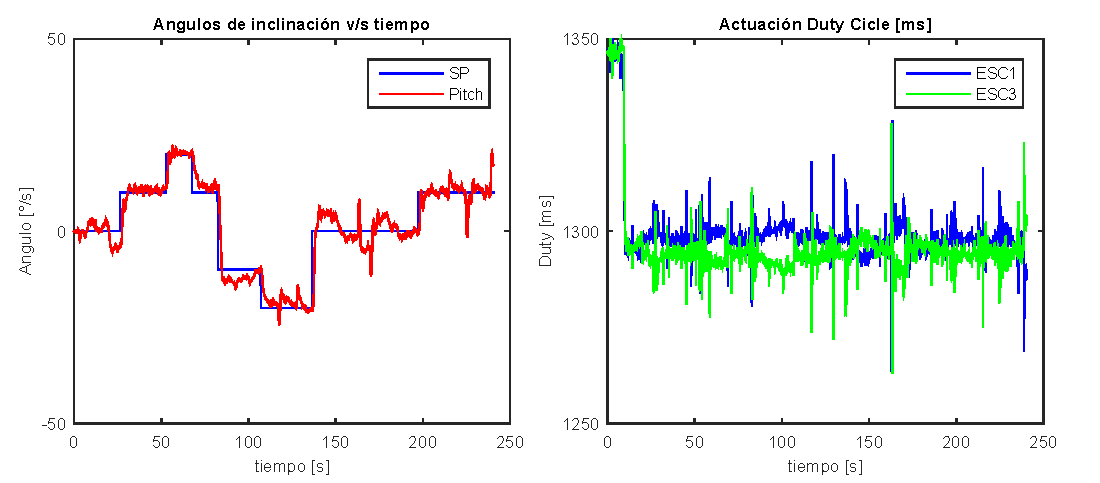
\includegraphics[scale=0.8]{PitchMadera}
	\par\end{centering}
	\caption{Estabilización eje Pitch en Soporte de Madera}\label{fig: Resultado Pitch Grafico Ma}\noindent
	\end{figure}

	En primer lugar se mantiene la posición deseada en cero mientras se
	asignan los valores de integración a los controladores PID. Dichos
	valores no se dejan activos desde un comienzo debido a que mientras
	se elimina el offset de los sensores, la parte integrativa acumula
	error, saturando el sistema al momento de encender los motores. El
	experimento prosigue con el cambio de posiciones angulares a +10$\degree$,
	+20$\degree$, +10$\degree$, -10$\degree$
	y $-20$. Donde se puede observar que el vehículo tiende a seguir
	las referencias constantes. Luego de que está en la posición de -20$\degree$,
	se perturba el sistema, verificando que vuelve a la posición deseada.
	Luego se fija un setpoint de cero grados para inducir nuevamente dos
	perturbaciones al sistema, finalizando con un cambio de posición a
	+10$\degree$ donde nuevamente se perturba el sistema verificando
	que vuelve a estabilizarse cerca de los valores deseados.

	\item \textbf{Resultados Roll}

	Siguiendo el mismo método experimental de sintonización de los parámetros,
	se somete a prueba el eje Roll, cuyos resultados se presentan en la tabla \ref{table: Parametros Roll Ma} y en la figura \ref{fig: Resultados Roll Grafico Ma}.

	\begin{table}[H]
	\noindent \begin{centering}
	\begin{tabular}{|c|c|c|}
	\hline 
	Parámetros PID & PID Interno & PID Externo\tabularnewline
	\hline 
	\hline 
	$Kp$ & 0.6 & 1\tabularnewline
	\hline 
	$K_{i}$ & 0.8 & 0.1\tabularnewline
	\hline 
	$K_{d}$ & 0.004 & 0.004\tabularnewline
	\hline 
	\end{tabular}
	\par\end{centering}
	\caption{Parámetros de los controladores PID Roll.}\label{table: Parametros Roll Ma}\noindent
	\end{table}

	\begin{figure}[H]
	\noindent \begin{centering}
	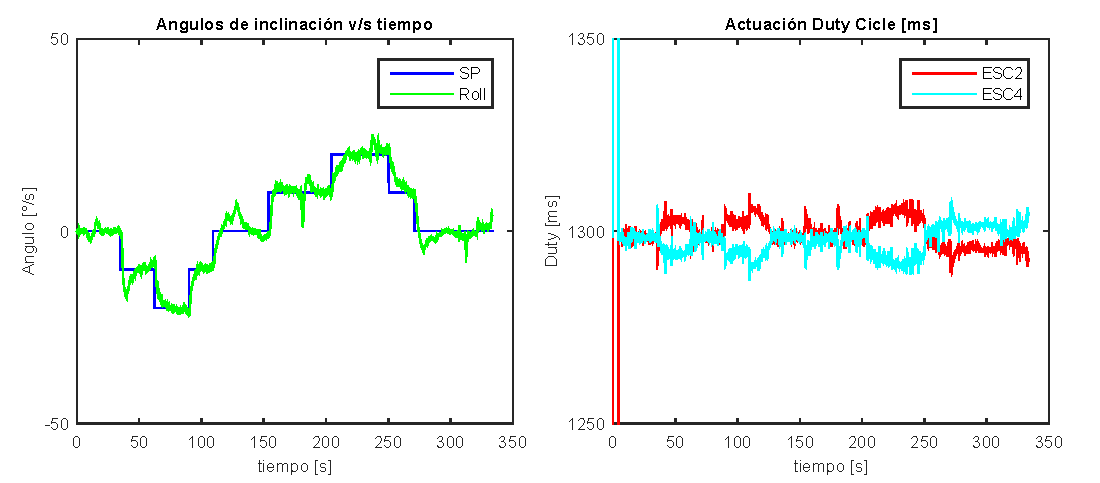
\includegraphics[scale=0.8]{RollMadera}
	\par\end{centering}
	\caption{Estabilización eje Roll en Soporte de Madera.}\label{fig: Resultados Roll Grafico Ma}\noindent
	\end{figure}

	El experimento también comienza calculando el offset asociado a los
	sensores, por lo tanto también se fijan los valores de integración
	después de esta etapa. En primer lugar se comienza con el vehículo
	estable en la posición cero, para cambiar referencia a -10$\degree$, 
	-20$\degree$, -10$\degree$ y 0$\degree$,
	con el fin de verificar seguimiento. Posteriormente se realizan los
	mismos cambios de referencia en sentido contrario, induciendo perturbación
	en +10$\degree$ y en +20$\degree$ cuyo
	resultado es que el vehículo vuelve a la posición deseada. Una vez
	que se vuelve a la posición cero, también se inducen perturbaciones
	verificando que el vehículo vuelve a la estabilización en dicha posición.
\end{enumerate}

\subsubsection{Estabilización de Eje Pitch, Roll y Yaw en soporte 2}

Antes de probar la estabilización del vehículo en vuelo hovering,
se somete a pruebas experimentales sobre el soporte de metal con tres
grados de libertad descrito en el Capítulo \ref{Componentes del Sistema} Componentes del Sistema. En primera
instancia es necesario mencionar las características del soporte que
impiden ajustar el controlador aplicado en la simulación. La primera
es que el centro de masa del vehículo sobre el soporte no es el que
se considera para el modelo del mismo en el Capítulo \ref{Modelado de la Planta} Modelo de la Planta, puesto que
el soporte construido a partir de una junta cardánica deja el quadcopter
en una posición similar a un péndulo invertido. La otra característica
desfavorable para fines de control, es el elevado roce que presentan
los rodamientos de la estructura, dificultando el seguimiento de referencias
constantes y la robustez a perturbaciones. La figura \ref{fig:Carac_soport}\textbf{
} muestra de mejor forma lo mencionado anteriormente, donde CQ es el centro de masa del Quadcopter y CC es el centro del cardán sobre el que gira.

\begin{figure}[H]
\noindent \begin{centering}
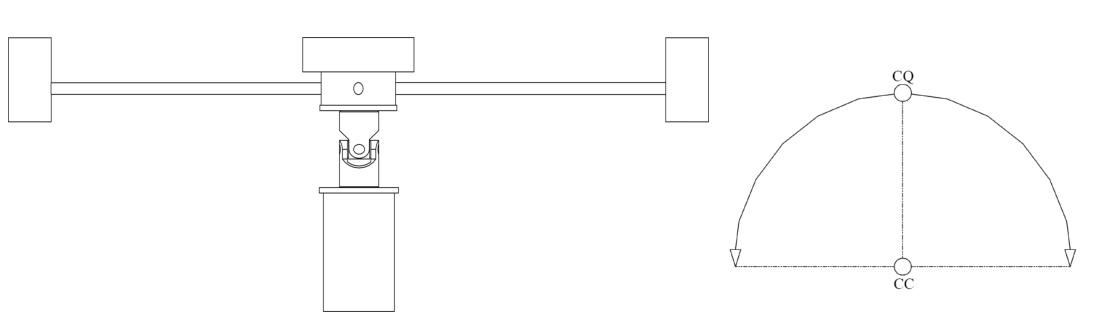
\includegraphics[scale=0.8]{SoporteCM}
\par\end{centering}
\caption{Características del soporte de metal.\label{fig:Carac_soport}}
\end{figure}


Por lo tanto, sobre éste soporte se aplica la estrategia de control
en cascada al igual que en el soporte de madera, obteniendo resultados
en el control de cada eje por separado, pero no así en el control
del vehículo completo, es decir, con todos sus ejes libres. Los resultados
experimentales se describen a continuación.

\begin{enumerate}
	\item \textbf{Resultados Pitch}
	Para la sintonización de los parámetros de los controladores PID se
	siguen los mismos pasos descritos en la estabilización con el soporte
	de madera. Dadas las limitaciones del diseño del soporte de metal, las pruebas
	de estabilización son un tanto diferentes para los ejes de Pitch y
	Roll. Éstas solo contemplan la estabilización sobre la referencia
	en cero, dado que por el alto roce no es posible realizar seguimiento
	sin saturar la actuación o sin que la planta oscile de manera violenta,
	agregando peligro para las personas en las pruebas. Otra diferencia es la respuesta
	del sistema a las perturbaciones en la posición angular, dado que
	el vehículo solo vuelve a la posición deseada ante pequeñas perturbaciones,
	si estas aumentan en intensidad, el vehículo no contraresta el movimiento
	aplicado de manera correcta en gran parte por las condiciones del
	soporte.

	Los resultados de las pruebas de estabilización sobre el eje Pitch
	se presentan en la tabla \ref{table: Parametros Pitch Me} y en la figura \ref{fig: Resultados Pitch Me} :

	\begin{table}[H]
	\noindent \begin{centering}
	\begin{tabular}{|c|c|c|}
	\hline 
	Parámetros PID & PID Interno & PID Externo\tabularnewline
	\hline 
	\hline 
	$Kp$ & 2.2 & 1.8\tabularnewline
	\hline 
	$K_{i}$ & 0.8 & 0.6\tabularnewline
	\hline 
	$K_{d}$ & 0.006 & 0.005\tabularnewline
	\hline 
	\end{tabular}
	\par\end{centering}
	\caption{Parámetros de los controladores PID Pitch.}\label{table: Parametros Pitch Me}\noindent
	\end{table}

	\begin{figure}[H]
	\noindent \begin{centering}
	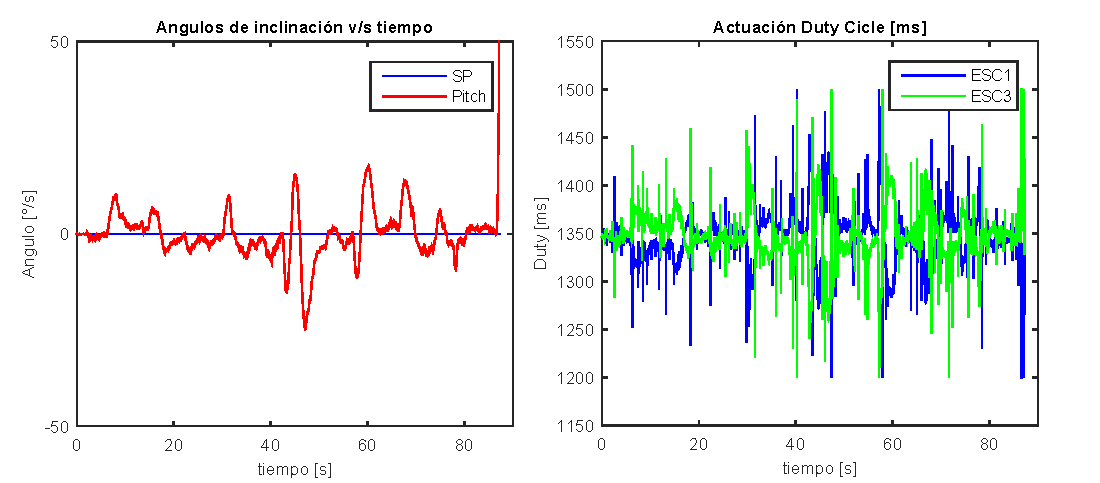
\includegraphics[scale=0.8]{PitchMetal}
	\par\end{centering}
	\caption{Estabilización eje Pitch en Soporte de Metal 3DOF.}\label{fig: Resultados Pitch Me}\noindent
	\end{figure}

	El experimento comienza con el quadcopter en la posición de equilibrio
	para eliminar el offset de los sensores. Como las pruebas contemplan
	la estabilización en la posición cero, se procede a perturbar el sistema
	manualmente con diferentes intensidades, baja, media y alta. A los 17{[}s{]} se aplica la primera
	perturbación de pequeña magnitud, al igual que a los 24{[}s{]} en
	sentido contrario, posteriormente a los 33{[}s{]} y 43{[}s{]} empujando
	el vehículo con fuerza moderada. Ante todas las perturbaciones anteriores
	el vehículo vuelve cerca de la posición deseada de estabilidad. 

	Luego se aumenta la fuerza externa aplicada a los 46{[}s{]}, 63{[}s{]}
	y 72{[}s{]} de comenzado el experimento, cuyo efecto es la inestabilidad
	y saturación de la actuación, donde el vehículo alcanza los límites
	máximos de desplazamiento angular permitidos por el soporte y el tren
	de aterrizaje. Después de la inestabilidad provocada por la perturbación,
	el vehículo es capaz de retomar su posición estable, pero sin duda
	no es el resultado esperado dado el tiempo que transcurre entre ambas
	y los desplazamientos angulares alcanzados, que de no estar limitados,
	serían aún mayores.

	\item \textbf{Resultados Roll}
	Tomando las mismas consideraciones que para las pruebas experimentales
	con el eje Pitch, se presentan los resultados obtenidos para la estabilización
	sobre el soporte de metal para el eje Roll, que se muestra en la tabla \ref{table: Parametros Roll Me} y en la figura \ref{fig:Estabilizacion-eje-Roll}.

	\begin{table}[H]
	\noindent \begin{centering}
	\begin{tabular}{|c|c|c|}
	\hline 
	Parámetros PID & PID Interno & PID Externo\tabularnewline
	\hline 
	\hline 
	$Kp$ & 1.8 & 2.2\tabularnewline
	\hline 
	$K_{i}$ & 0.8 & 0.8\tabularnewline
	\hline 
	$K_{d}$ & 0.004 & 0.004\tabularnewline
	\hline 
	\end{tabular}
	\par\end{centering}
	\caption{Parámetros de los controladores PID.}\label{table: Parametros Roll Me}
	\end{table}

	\begin{figure}[H]
	\noindent \begin{centering}
	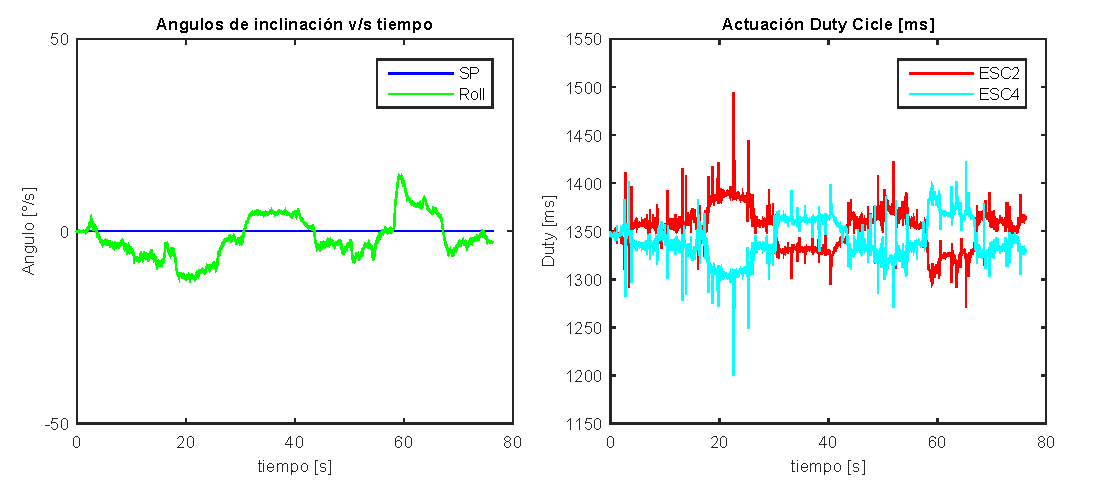
\includegraphics[scale=0.8]{RollMetal}
	\par\end{centering}
	\caption{Estabilización eje Roll en Soporte de Metal 3DOF.\label{fig:Estabilizacion-eje-Roll}}
	\end{figure}

	En esta oportunidad el experimento se hace en el eje del soporte que
	presenta mayor roce. Ésto se hace evidente al observar el comportamiento
	del vehículo luego de ser perturbado. De la figura \ref{fig:Estabilizacion-eje-Roll}
	se puede observar que cada vez que se perturba el sistema, el vehículo
	demora más de 10 segundos en retomar posiciones angulares cercanas
	al punto deseado. Un ejemplo claro es la perturbación inducida transcurridos
	13{[}s{]}, donde el vehículo logra retomar su posición de estabilidad
	cerca de los 30{[}s{]}, donde se perturba otra vez en dirección contraria
	para observar el mismo comportamiento. Es importante mencionar que
	la causa principal de este comportamiento se debe al roce del soporte,
	dado que las acciones de control se pueden apreciar claramente en
	el gráfico de actuación, cuyas diferencias en ciclo de trabajo generan
	el torque suficiente para estabilizar rápidamente con un coeficiente
	de roce menor.

	\item \textbf{Resultados Yaw}

	Para poner a prueba el control estabilizador en el eje Yaw, se bloquea
	el movimiento de los dos ejes anteriormente descritos. El soporte
	inspirado en una junta cardánica tiene un rodamiento en su base, el
	cual le permite girar en torno al eje $z$ del sistema cartesiano. 

	En este experimento el vehículo montado sobre el soporte concuerda
	con el modelo descrito en el Capítulo \ref{Modelado de la Planta} Modelado de la Planta, dado que en este caso el giro
	se produce en torno al eje que pasa por el centro de masa del vehículo,
	obteniendose resultados razonables para el seguimiento de referencias. 

	La principal desviación durante el desarrollo del experimento, es
	la obtención de la posición angular por medio de la integración de
	las mediciones del gyroscopo, dado que el error del mismo sensor sumado
	al ruido de los motores, distorciona el punto de partida del vehículo,
	lo que se puede apreciar en los videos demostrativos, no así en los
	gráficos que registran la posición angular.

	Los resultados obtenidos se muestran en la tabla \ref{table: Parametros Yaw Me} y en la figura \ref{fig: Resultados Yaw Me} :

	\begin{table}[H]
	\noindent \begin{centering}
	\begin{tabular}{|c|c|c|}
	\hline 
	Parámetros PID & PID Interno & PID Externo\tabularnewline
	\hline 
	\hline 
	$Kp$ & 2.6 & 6\tabularnewline
	\hline 
	$K_{i}$ & 0 & 0.01\tabularnewline
	\hline 
	$K_{d}$ & 0.002 & 0.004\tabularnewline
	\hline 
	\end{tabular}
	\par\end{centering}
	\caption{Parámetros de los controladores PID Yaw.}\label{table: Parametros Yaw Me}\noindent
	\end{table}

	\begin{figure}[H]
	\noindent \begin{centering}
	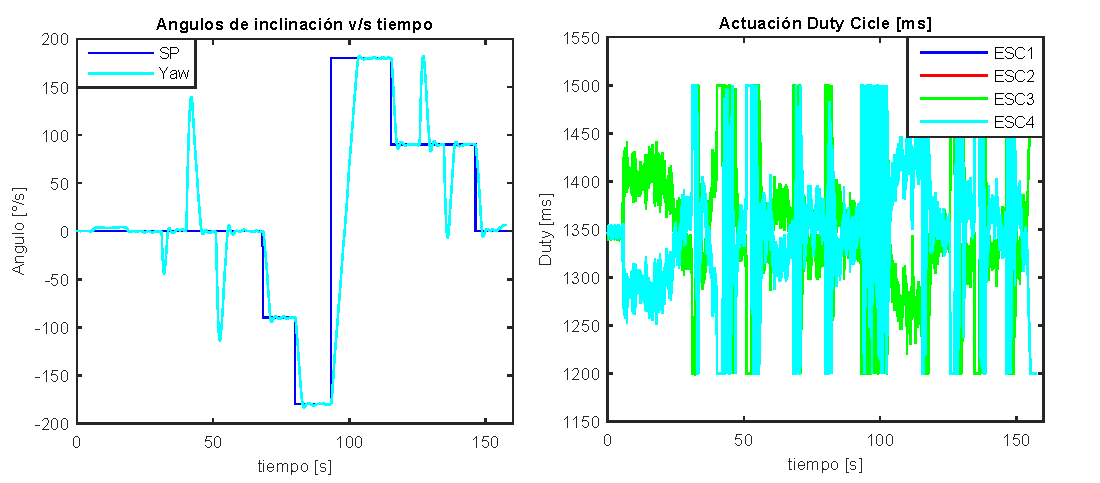
\includegraphics[scale=0.8]{YawMetal}
	\par\end{centering}
	\caption{Estabilización eje Yaw en Soporte de Metal 3DOF.}\label{fig: Resultados Yaw Me}\noindent
	\end{figure}

	Del experimento es claro observar que el ángulo Yaw se mantiene estable
	en el punto de operación. Después de aplicar perturbaciones al sistema
	en 27{[}s{]}, 34{[}s{]} y 42{[}s{]} el sistema se estabiliza otra
	vez cerca de los puntos de referencia. Es claro que mientras mayor
	sea la perturbación, mayor es el tiempo que toma estabilizar el vehículo.
	Del gráfico anterior también se puede observar el seguimiento de referencias
	constantes, donde también se puede perturbar el sistema y volver a
	la posición deseada sin problemas. El detalle en este experimento
	es la desviación en la posición original cero grados al inicio de
	las pruebas, con la posición cero al final de estas, ambas son diferentes
	dado el error acumulativo de integrar las mediciones del gyroscopo
	para obtener dicha posición. Ésta desviación no es apreciable por medio de gráficos, pero sí se puede 		observar en las grabaciones de video realizadas para la presentación del proyecto de titulación.
\end{enumerate}
\end{document}
